% =====================================================================
%  P3 GROUP REPORT -- "On the Habitability of Titan"
%  Cross-disciplinary synthesis of five individual reports.
%
%  Formatting per brief: >= 11pt Arial, 1.5 line spacing, <= 3000 words
%  (main text, excluding the abstract, captions, and bibliography).
%
%  PARENT DOCUMENT. Section content lives in the child files:
%    abstract.tex, subsurface.tex (Charlotte), craters.tex (Helena),
%    brine.tex (Lucca), surface.tex (Chris), atmosphere.tex (Imaan).
%  Each group member edits their own file; the Introduction and Outlook
%  live here and are shared.
% =====================================================================
\documentclass[11pt,a4paper]{article}

% ---- Arial substitute: Helvetica via helvet, set as the default family
\usepackage[T1]{fontenc}
\usepackage{helvet}
\renewcommand{\familydefault}{\sfdefault}

\usepackage[a4paper,margin=2.5cm]{geometry}
\usepackage{setspace}
\onehalfspacing                     % 1.5 line spacing
\usepackage{graphicx}
\graphicspath{{images/}}
\usepackage[labelfont=bf,font=small]{caption}
\usepackage[round]{natbib}
\bibliographystyle{plainnat}
\usepackage{xcolor}
\usepackage[colorlinks=true,allcolors=blue!55!black]{hyperref}

% Visual marker for content still to be supplied by a group member.
\newcommand{\placeholder}[1]{\par\medskip\noindent\textcolor{gray}{\itshape [#1]}\par\medskip}

\setlength{\parskip}{0.4em}
\setlength{\parindent}{0pt}

\title{\textbf{On the Habitability of Titan:\\ A Cross-Disciplinary Synthesis}}
\author{L.\ M.\ Castlevetro, C.\ Crick, C.\ Meadows, H.\ R.\ Nicolaides, I.\ S.\ Islam Rahim\\[2pt]
\normalsize MPhil in Planetary Science and Life in the Universe, University of Cambridge}
\date{July 2026}

\begin{document}
\maketitle

% ---- Abstract (does not count towards the 3000-word limit) ----
% ---- Abstract (<= half a page; excluded from the 3000-word limit) ----
\begin{abstract}
\noindent
Titan presents a rare combination of a dense, organic-rich atmosphere, stable surface liquids, an
abundant supply of prebiotic feedstock, and a probable subsurface water ocean, making it one of the
foremost astrobiological targets in the Solar System. Yet its habitability is constrained by the
physical separation of liquid water from surface organics, and by growing uncertainty over whether a
subsurface ocean survives at all. This group report synthesises five complementary studies that
together span Titan from its silicate core to its upper atmosphere: the tidal heating and thermal
evolution of the interior ocean; impact-driven melt production within the ice shell; prebiotic
reaction chemistry in transient impact brine pockets; longitudinal, seasonal structure in the
atmosphere; and a Bayesian, time-resolved map of surface habitability. Read together, these studies
identify impact cratering as a key process bridging Titan's isolated reservoirs, and geological time
as the axis along which its habitability rises and falls. We find that Titan offers multiple, largely
independent candidate habitats -- surface, ice-shell, and interior -- whose viability does not stand
or fall on the ocean question alone. We close with a combined outlook for Titan's habitability and the
tests that the forthcoming Dragonfly mission will provide.
\end{abstract}


% =====================================================================
% ---- Introduction (shared; counts towards the 3000-word limit) ----
\section{Introduction}

Titan, Saturn's largest moon, is among the most compelling astrobiological targets in the Solar
System. The emergence of life as we understand it requires three ingredients in one place: a liquid
solvent, a supply of organic building blocks spanning the biogenic elements (CHNOPS), and a sustained
source of energy \citep{Maruyama2019}. Titan is the only body besides Earth known to host stable
surface liquids -- though its lakes and seas are methane and ethane rather than water -- and the only
moon with a dense, organic-rich atmosphere \citep{Sohl2014}. Photochemistry in that atmosphere
generates complex nitrogen-bearing organics, or tholins, along with prebiotic feedstock molecules such
as hydrogen cyanide \citep{Raulin2008}. Beneath roughly 100\,km of water ice, Cassini gravity and
rotation measurements inferred a global subsurface water ocean \citep{Iess2012, Durante2019}, an
environment that would satisfy the solvent requirement directly.

The central obstacle to Titan's habitability is not a shortage of ingredients but their separation.
Organics accumulate at the surface and in the atmosphere, while liquid water lies kilometres below an
insulating ice shell; the two rarely meet. Moreover, the very existence of the ocean is now contested:
recent re-analyses argue that Titan's measured tidal dissipation is too large to be compatible with a
decoupled liquid layer \citep{Petricca2025}, while others infer only a low-density ocean from a
reduced Love number \citep{Goossens2024}. Whether, where, and when Titan brings solvent, organics, and
energy together therefore remains genuinely open.

This report addresses that overarching question through five complementary, cross-disciplinary studies
that together span Titan from its silicate core to its upper atmosphere, following the layered
structure of Figure~\ref{fig:crosssection}. Working outward from the deep interior, Crick
\citep{Crick2026} models tidal heating and the thermal survival of the subsurface ocean; Nicolaides
\citep{Nicolaides2026} quantifies impact-generated melt production in the ice shell over Titan's
bombardment history; Castlevetro \citep{Castlevetro2026} simulates prebiotic chemistry within the
transient brine pockets those impacts create; and Islam Rahim \citep{IslamRahim2026} characterises
longitudinal and temporal structure in the organic-rich atmosphere. Meadows \citep{Meadows2026} then
draws these threads together at the surface, mapping the probability of habitability across the globe
and through geological time. Impact cratering emerges as a connective process linking these layers,
since it can excavate liquid water, mix in surface and cometary organics, and deliver both to depth
\citep{Thompson1992, Neish2024}.

\begin{figure}[htbp]
  \centering
  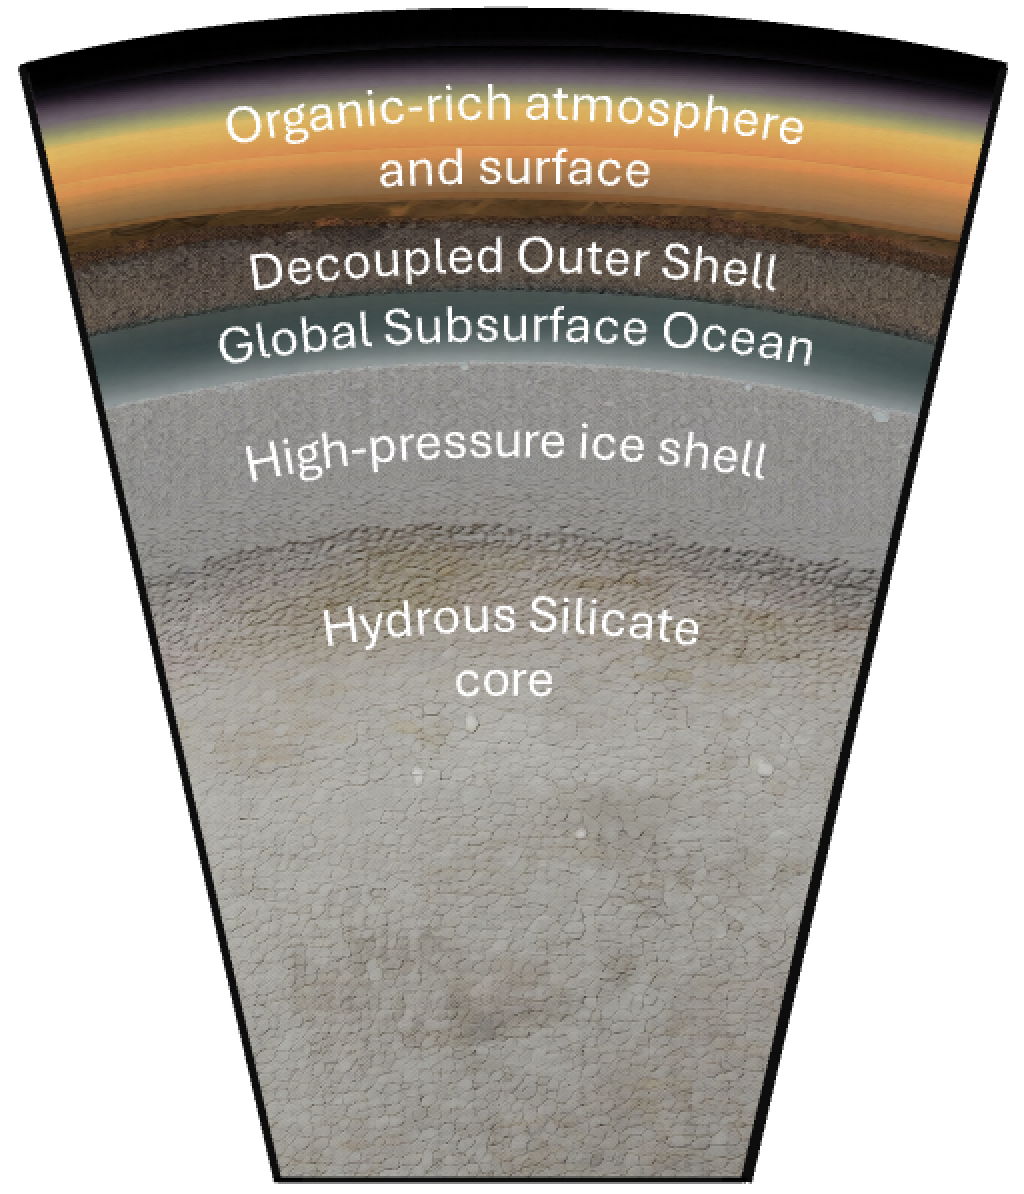
\includegraphics[width=0.5\linewidth]{images/titan_cross_section.png}
  \caption{Schematic cross-section of Titan's interior, from the hydrous silicate core through the
    high-pressure ice shell, the (contested) global subsurface ocean, and the decoupled outer ice
    shell, to the organic-rich surface and atmosphere. This report is organised around these layers:
    each of the five studies addresses habitability within one layer, or the exchange of material and
    energy between them, working from the interior outward. The figure provides the shared spatial
    frame for the summaries that follow.}
  \label{fig:crosssection}
\end{figure}

A second unifying theme is time. Titan's habitability is not static: the bombardment flux, the interior
thermal state, the surface insolation, and the atmosphere have all evolved from the Late Heavy
Bombardment towards the far future, when a red-giant Sun will warm the surface. The NASA Dragonfly
mission, arriving in 2034, will test many of these ideas directly at Selk crater \citep{Lorenz2021Landing}. In
the sections that follow we summarise the key insight from each study in turn, before synthesising them
into a combined outlook for Titan's habitability.


% =====================================================================
\section{Summary of the key insights from individual reports}

% ============================================================
\section{Subsurface Oceans: Orbital Evolution and Tidal Energy}
\label{sec:subsurface}
% ============================================================
\placeholder{Charlotte}


   % Charlotte -- interior / subsurface ocean
% ---- Helena: ice-shell impact melt production ----
\subsection{Impact melt production in the ice shell (Helena)}

\placeholder{Helena}
      % Helena    -- ice-shell impact melt
% ---- Lucca: prebiotic chemistry in impact brine pockets ----
\subsection{Prebiotic chemistry in impact brine pockets (Lucca)}

\placeholder{Lucca subsection}
        % Lucca     -- brine-pocket chemistry
% ---- Imaan: atmospheric longitudinal / temporal structure ----
\section{Longitudinal and temporal structure of the atmosphere }

\placeholder{Imaan}
   % Imaan     -- atmosphere
% ---- Chris: Bayesian surface habitability mapping ----
\subsection{Surface habitability mapping (Chris)}

My study asks a spatial question that the other four do not: \emph{where} is Titan's surface most likely
to be habitable, and how has that pattern changed through time? Working at the outermost layer of
Figure~\ref{fig:crosssection}, I cast this as Bayesian inference, computing a posterior habitability
probability $P(H)$ for every pixel of a global equirectangular grid ($\sim$$6.5\times10^{6}$ pixels at
4490\,m per pixel, for Titan's radius of 2575\,km). Eight geomorphological and compositional features
-- including liquid-hydrocarbon coverage, organic (VIMS) spectral signatures, geomorphological
diversity, and a methane-cycle proxy -- update a beta-conjugate prior, so that each map carries a
calibrated uncertainty rather than a single score \citep{Meadows2026}; surface temperatures follow
\citet{Jennings2019}.

The framework is applied at five epochs, from the Late Heavy Bombardment ($-3.5$\,Gya) to a red-giant
future ($+5.9$\,Gya), turning a static map into a trajectory. At present the north-polar lake shores
dominate the ranking: the liquid-hydrocarbon feature raises both the maximum and the spread of $P(H)$,
and the north-polar-to-equatorial contrast is the largest of any epoch (Figure~\ref{fig:habmap}). Selk
crater -- the Dragonfly landing site -- in fact scores only modestly ($P(H)\approx0.21$, against
$\sim0.55$ for the leading polar lakes), because the map measures present-day \emph{solvent}
habitability whereas Dragonfly targets \emph{past} liquid-water chemistry; the framework instead
endorses the mission through Selk's geomorphological diversity, the highest of any equatorial site and a
proxy for the organic--water-ice contact terrain it will sample \citep{Lorenz2021}. The global median
$P(H)$ climbs from $0.27$ at the LHB to $0.32$ at present, holds through the near-future plateau
($r>0.999$), then -- after a $\sim$1\,Gyr solvent-free minimum around $+5$\,Gya, once the hydrocarbon
seas evaporate -- rises to its maximum of $0.53$ under a red-giant water--ammonia ocean. Habitability is
therefore episodic in time; spatially, the lowest scores fall on the water-ice-rich cores of Xanadu and
the mountain ranges.

A deliberate strength is that the map is \emph{ocean-agnostic}: it scores the surface on its own
evidence, and so remains valid whether or not Titan retains the contested subsurface ocean
\citep{Petricca2025}, making it a robust anchor for the group's argument. It also indexes the other
studies: my top sites are polar lake shores, where present-day solvent and organics coincide, whereas
the impact melt pools of Nicolaides \citep{Nicolaides2026} and the brine pockets of Castlevetro
\citep{Castlevetro2026} form a complementary, largely equatorial class of liquid-water habitat that the
map flags through geomorphological diversity (as at Selk). The organic and methane-cycle features
driving the scores are supplied by the atmosphere Islam Rahim \citep{IslamRahim2026} shows to be
variable, while the deep energy budget is set by the interior Crick \citep{Crick2026} models. The
surface map thus points to \emph{where} the processes described by the rest of the group are most likely
to matter.

\begin{figure}[htbp]
  \centering
  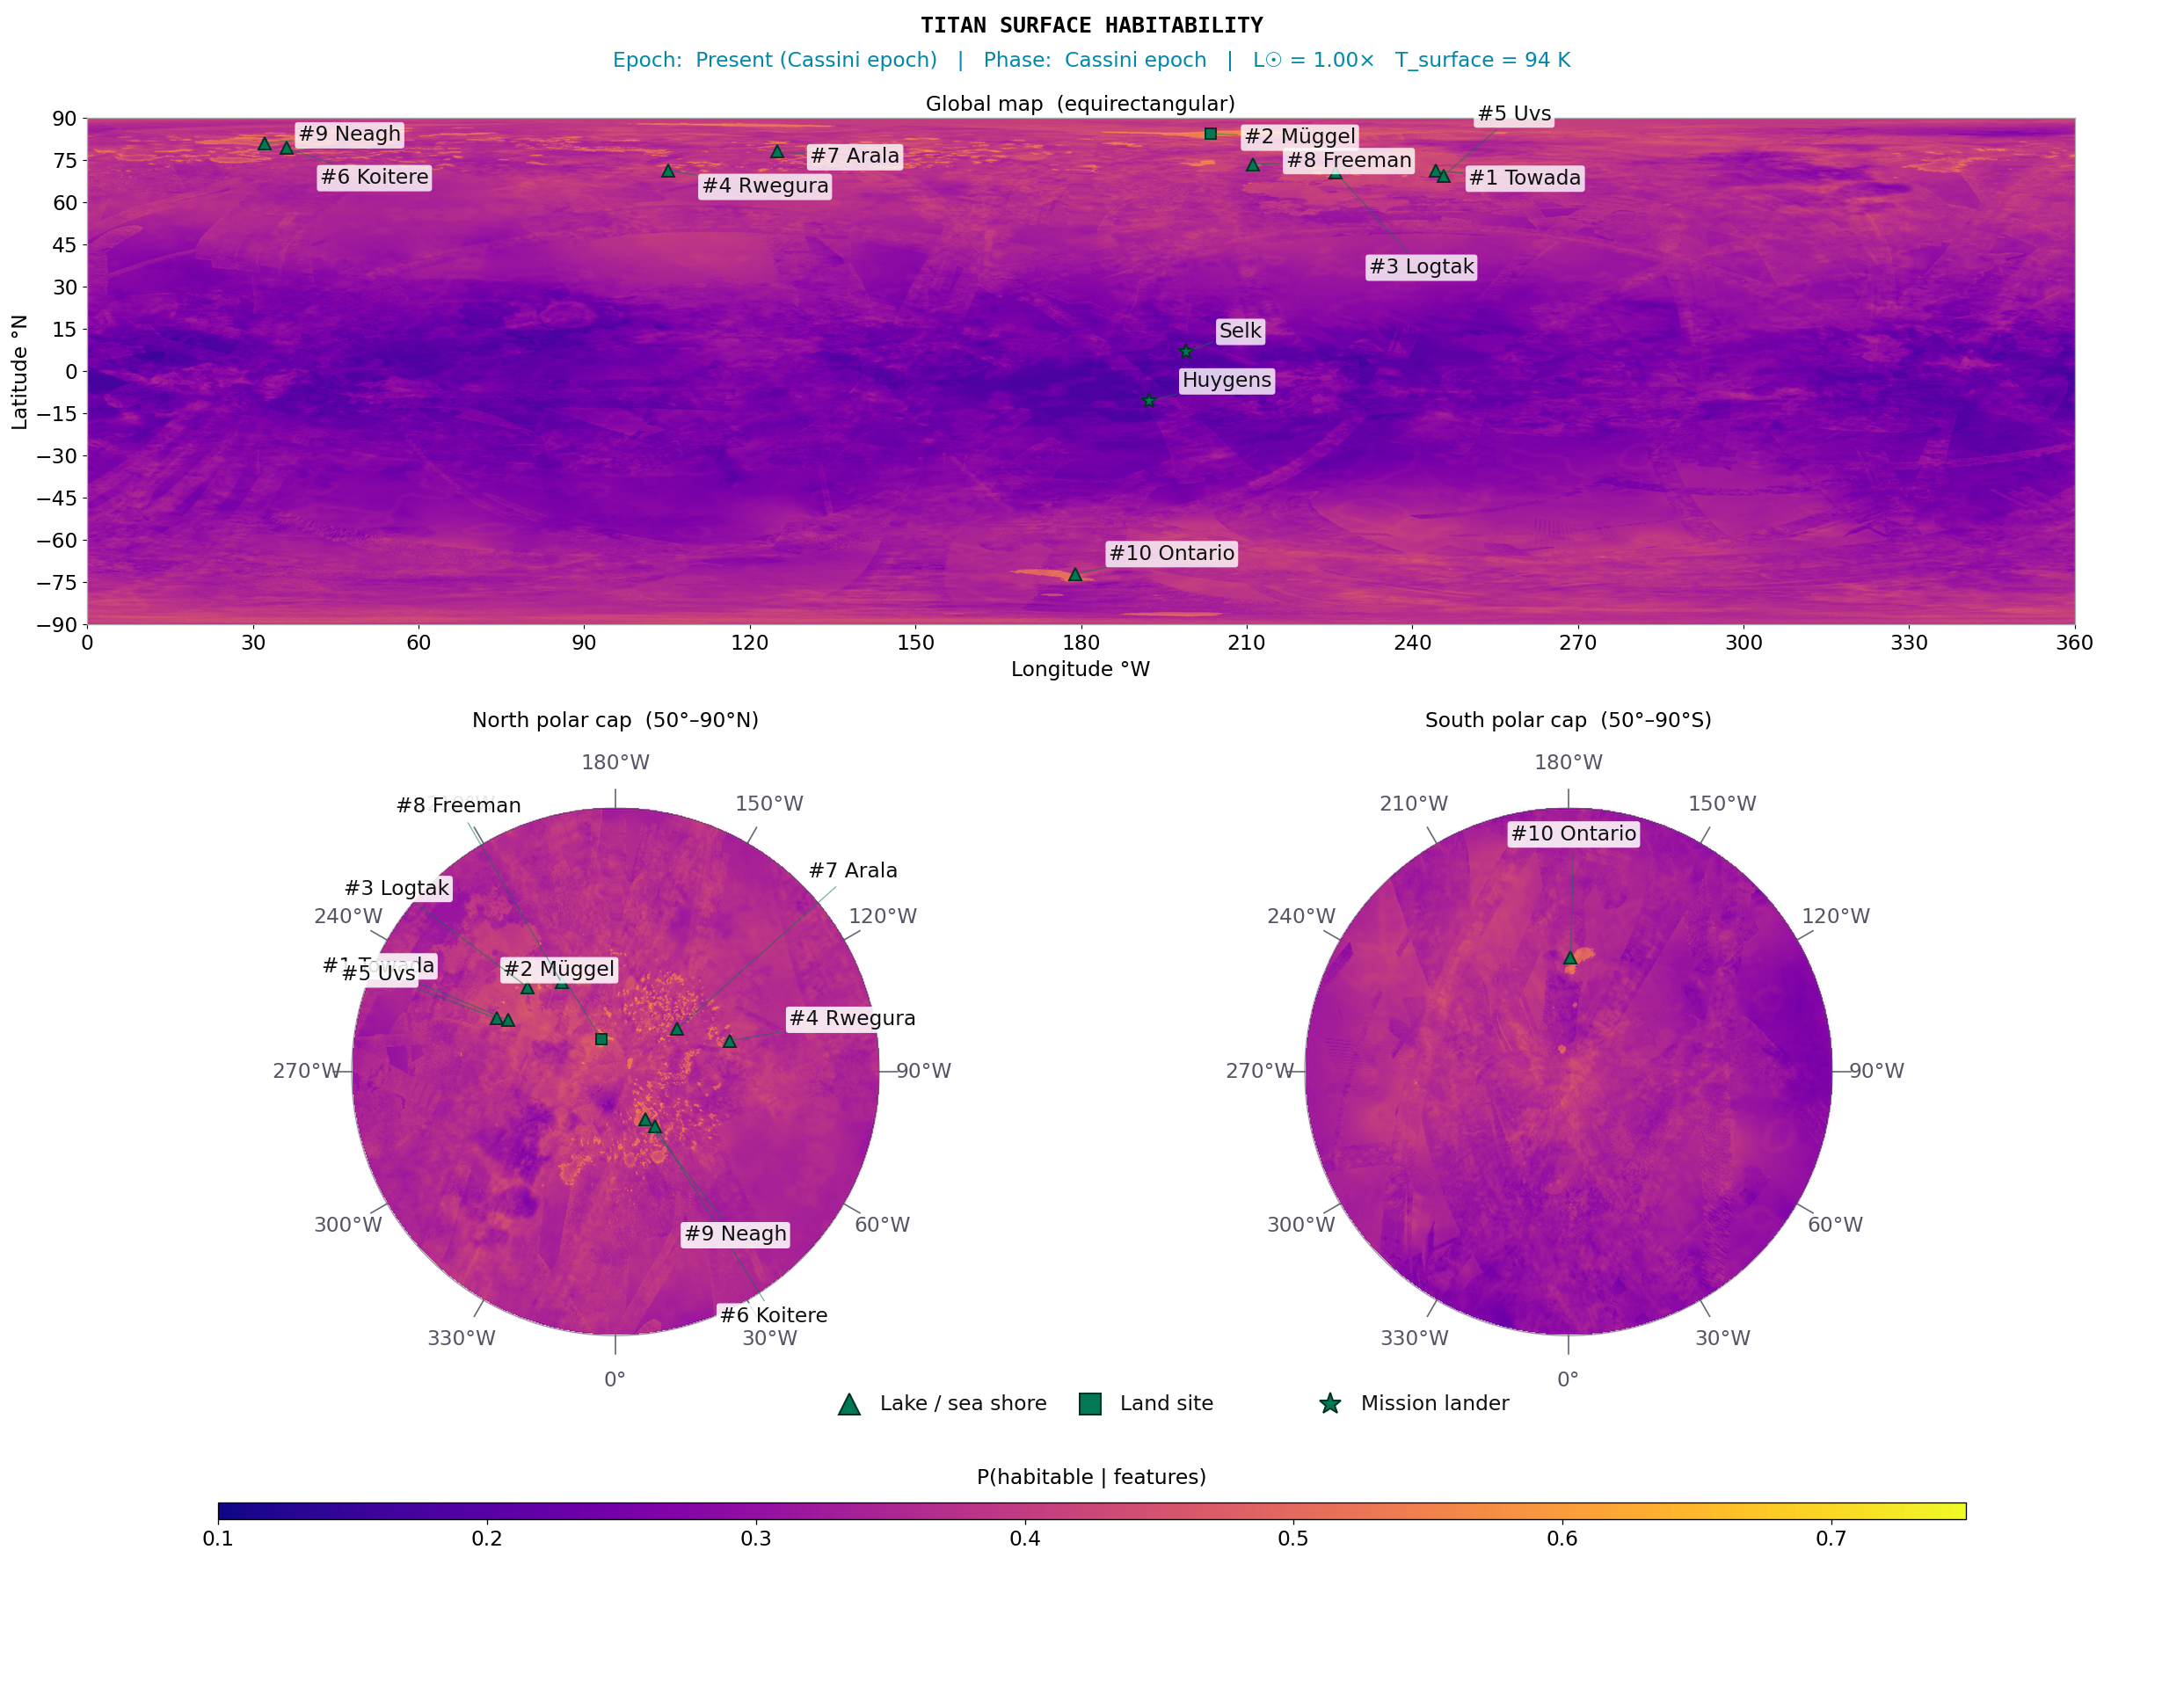
\includegraphics[width=\linewidth]{habitability_map.png}
  \caption{Present-epoch (Cassini era) posterior mean surface habitability map, $P(H)$, from the
    Bayesian framework of \citet{Meadows2026}. North-polar lake shores (top) attain the highest
    habitability probability; the radar-bright, water-ice-rich terrain of Xanadu and the mountain
    ranges score lowest. Selk crater (equatorial), the Dragonfly landing site, scores only
    modestly on this present-day solvent metric; the map instead endorses the mission's choice via
    Selk's high geomorphological-diversity feature.}
  \label{fig:habmap}
\end{figure}
      % Chris     -- surface habitability map

% =====================================================================
% ---- Outlook for habitability (joint synthesis) ----
\section{Outlook for habitability}

Taken together, the five studies make a layered rather than a singular case for Titan's habitability,
and point to one explicit conclusion: the most promising sites for prebiotic chemistry are the
liquid-water environments that impacts create. Impact melt pools -- and the subsurface ocean, if it
persists -- are the principal settings that bring liquid water into contact with Titan's abundant
surface organics \citep{Nicolaides2026, Crick2026}, and reactive simulations show that such a brine
spontaneously forms carbon--nitrogen bonds, mobilises amino acids, and incorporates phosphorus and
sulphur: the first steps of prebiotic chemistry \citep{Castlevetro2026}.

This potential is contingent, not guaranteed. Whether a given impact yields a viable reactor depends on
the ambient conditions when it occurs: the impactor's size, speed and angle set how much organic
feedstock survives atmospheric entry and shock, while the impact energy, target composition and epoch
set the melt volume and the pocket's freezing lifetime \citep{Nicolaides2026}. Habitability on Titan is
therefore episodic and site-specific rather than global.

Most speculatively, wherever liquid water endures -- the ocean, or long-lived melt lenses such as that
beneath Selk crater -- Titan could host anaerobic, methanogen-like life, whose biogenic methane is even
one candidate explanation for the moon's otherwise puzzling atmospheric supply \citep{IslamRahim2026}.
NASA's Dragonfly mission (2034) will sample impact-altered organics directly at Selk crater -- the
equatorial site our map singles out for its organic--ice contact terrain \citep{Lorenz2021,
Meadows2026} -- offering a first test; JWST can extend the
atmospheric record, while resolving the ocean question ultimately requires a dedicated gravity orbiter.
Should a red-giant Sun ultimately warm the surface, Titan's most habitable chapter may still lie ahead.
    % joint synthesis and forward look

% =====================================================================
\bibliography{references}

\end{document}
